\documentclass{beamer}
\usetheme{tokitex}

\usepackage{graphics}
\usepackage{multirow}
\usepackage{tabto}

\usepackage[english,bahasa]{babel}
\newtranslation[to=bahasa]{Section}{Bagian}
\newtranslation[to=bahasa]{Subsection}{Subbagian}

\usepackage{listings, lstautogobble}
\usepackage{color}

\definecolor{dkgreen}{rgb}{0,0.6,0}
\definecolor{gray}{rgb}{0.5,0.5,0.5}
\definecolor{mauve}{rgb}{0.58,0,0.82}

\lstset{frame=tb,
  language=pascal,
  aboveskip=1mm,
  belowskip=1mm,
  showstringspaces=false,
  columns=fullflexible,
  keepspaces=true,
  basicstyle={\small\ttfamily},
  numbers=none,
  numberstyle=\tiny\color{gray},
  keywordstyle=\color{blue},
  commentstyle=\color{dkgreen},
  stringstyle=\color{mauve},
  breaklines=true,
  breakatwhitespace=true,
  autogobble=true
}

\title{Pencarian}
\author{Tim Olimpiade Komputer Indonesia}
\date{}

\begin{document}

\begin{frame}
\titlepage
\end{frame}

\begin{frame}
\frametitle{Pendahuluan}
Melalui dokumen ini, kalian akan:
\begin{itemize}
  \item Mempelajari konsep algoritma sederhana.
  \item Memahami berbagai algoritma pencarian.
\end{itemize}
\end{frame}

\begin{frame}
\frametitle{Pendahuluan (lanj.)}
\begin{itemize}
  \item Pencarian merupakan hal sederhana dan sering digunakan dalam pemrograman.
  \item Terdapat berbagai macam cara untuk melakukan pencarian. 
  \item Membahas beberapa cara tersebut dapat memberikan gambaran bagaimana sebuah persoalan diselesaikan dengan berbagai algoritma.
\end{itemize}
\end{frame}

\begin{frame}
\frametitle{Soal: Sepatu Untuk Bebek}
Deskripsi:
\begin{itemize}
  \item Kwek, salah satu bebek Pak Dengklek akan segera merayakan ulang tahunnya. Pak Dengklek akan memberikan Kwek hadiah ulang tahun berupa sepatu.
  \item Terdapat $N$ sepatu di toko. Sepatu ke-$i$ memiliki ukuran sebesar $h_i$.
  \item Pak Dengklek tahu bahwa ukuran kaki Kwek adalah sebuah bilangan bulat $X$.
  \item Karena $N$ bisa jadi sangat besar, Pak Dengklek meminta bantuan kalian untuk mencari sepatu ke berapa yang cocok dengan ukuran kaki Kwek.
  \item Bantulah dia!
\end{itemize}
\end{frame}

\begin{frame}
\frametitle{Soal: Sepatu Untuk Bebek (lanj.)}
Format masukan:
\begin{itemize}
  \item Baris pertama berisi dua bilangan bulat, yaitu $N$ dan $X$.
  \item Baris kedua berisi $N$ bilangan bulat. Bilangan ke-$i$ menyatakan $h_i$.
\end{itemize}
Format keluaran:
\begin{itemize}
  \item Jika ada ukuran sepatu yang cocok, cetak sebuah baris yang menyatakan nomor sepatu yang cocok dengan ukuran kaki Kwek.
  \item Jika tidak ada ukuran sepatu yang cocok, cetak "beri hadiah lain".
\end{itemize}
Batasan:
\begin{itemize}
  \item $1 \le N \le 100.000$
  \item $1 \le X \le 100.000$
  \item $1 \le h_i \le 100.000$, untuk $1 \le i \le N$
\end{itemize}
\end{frame}

\begin{frame}
\frametitle{Solusi}
\begin{itemize}
  \item Kita dihadapkan pada persoalan pencarian: diberikan $N$ angka. Cari apakah $X$ ada di antara angka-angka tersebut.
  \item Jika ditemukan, cetak di urutan ke berapa angka tersebut berada.
  \item Salah satu ide yang muncul adalah:
  \begin{itemize}
    \item Periksa satu per satu dari sepatu pertama, kedua, ketiga, dan seterusnya.
    \item Jika ditemukan, langsung laporkan.
    \item Jika sampai akhir belum juga ditemukan, artinya angka yang dicari tidak ada pada daftar.
  \end{itemize}
\end{itemize}
\end{frame}

\begin{frame}[fragile]
\frametitle{Contoh Solusi: cari\_1.pas}
Implementasinya cukup sederhana:
\begin{lstlisting}
  (* pencarian *)
  hasil := 0; (* artinya belum ditemukan *)
  for i := 1 to N do begin
    if (h[i] = X) then begin
      hasil := i;
      break;
    end;
  end;

  if (hasil = 0) then begin
    writeln('beri hadiah lain');
  end else begin
    writeln(hasil);
  end;
\end{lstlisting}
\end{frame}

\begin{frame}
\frametitle{Solusi (lanj.)}
\begin{itemize}
  \item Algoritma pencarian dengan membandingkan elemen satu per satu semacam ini disebut dengan \alert{\textit{sequential search}} atau \alert{\textit{linear search}}.
  \item Jika ada $N$ elemen pada daftar yang perlu dicari, maka paling banyak diperlukan $N$ operasi perbandingan.
  \item Dalam kompleksitas waktu, performa algoritma \textit{sequential search} bisa dinyatakan dalam $O(N)$.
\end{itemize}
\end{frame}

\begin{frame}
\frametitle{Adakah yang Lebih Cepat?}
\begin{itemize}
  \item Misalkan terdapat 90.000 kata pada Kamus Besar Bahasa Indonesia (KBBI).
  \item Bayangkan jika sesekali kita butuh mencari arti kata pada kamus, dan dengan \textit{sequential search} perlu dilakukan paling banyak 90.000 operasi.
  \item Apakah kita sebagai manusia melakukan perbandingan sampai 90.000 kata?
\end{itemize}
\end{frame}

\begin{frame}
\frametitle{Adakah yang Lebih Cepat? (lanj.)}
\begin{itemize}
  \item Pada kehidupan nyata, sebagai manusia kita tidak mencari kata satu per satu, halaman demi halaman, sampai 90.000 kata.
  \item Bahkan, kita dapat mencari arti suatu kata cukup dalam beberapa perbandingan, yang jauh lebih sedikit dari 90.000.
  \item Bagaimana hal ini bisa terjadi?
\end{itemize}
\end{frame}

\begin{frame}
\frametitle{Properti Khusus: Terurut}
\begin{itemize}
  \item KBBI memiliki sebuah properti yang khusus, yaitu \alert{terurut berdasarkan abjad}.
  \item Dengan cara ini, kita bisa membuka halaman tengah dari KBBI, lalu periksa apakah kata yang kita cari ada pada halaman tersebut.
\end{itemize}
\end{frame}

\begin{frame}
\frametitle{Properti Khusus: Terurut (lanj.)}
\begin{itemize}
  \item Misalkan kata yang kita cari berawalan 'W', lalu halaman tengah hanya menunjukkan daftar kata dengan awalan 'G'. Jelas bahwa kata yang kita cari tidak mungkin berada di \alert{separuh pertama} kamus.
  \item Ulangi hal serupa dengan separuh belakang kamus, buka bagian tengahnya dan bandingkan.
  \item Dengan cara ini, setiap perbandingan akan mengeleminasi separuh rentang pencarian!
\end{itemize}
\end{frame}

\begin{frame}
\frametitle{Analisis Performa}
\begin{itemize}
  \item Misalkan terdapat sebuah daftar berisi $N$ elemen, dan kita perlu mencari salah satu elemen.
  \item Banyaknya operasi maksimal yang dibutuhkan sampai suatu elemen bisa dipastikan keberadaannya sama dengan panjang dari barisan $[N, \frac{N}{2}, \frac{N}{4}, \frac{N}{8}, ..., 2, 1]$
  \item Yaitu sebesar $\lceil ^2\log{N} \rceil$, sehingga kompleksitasnya $O(\log{N})$.
  \item Pencarian seperti ini disebut dengan \alert{\textbf{binary search}}
\end{itemize}
\end{frame}

\begin{frame}
\frametitle{Perbandingan dengan Sequential Search}
Perhatikan tabel banyaknya operasi yang dibutuhkan untuk nilai $N$ tertentu:
\begin{table}[ht]
  \begin{tabular}{|c|c|c|}
    \hline N  & Sequential  & Binary \\
    \hline 50 & 50 & 6 \\
    \hline 100 & 100 & 7 \\
    \hline 150 & 150 & 8 \\
    \hline 200 & 200 & 8 \\
    \hline 250 & 250 & 8 \\
    \hline 300 & 300 & 9 \\
    \hline
  \end{tabular}
\end{table}
Seperti yang terlihat, \textit{binary search} jauh lebih cepat!

Bahkan untuk $N = 10^6$, \textit{binary search} hanya butuh maksimal 20 operasi!
\end{frame}

\begin{frame}[fragile]
\frametitle{Implementasi (cari\_2.pas)}
Terdapat bermacam cara implementasi \textit{binary search}. Salah satunya:
\begin{lstlisting}
  (* pencarian *)
  hasil := 0; (* artinya belum ditemukan *)
  kiri := 1;
  kanan := N;
  while ((kiri <= kanan) and (hasil = 0)) do begin
    tengah := (kiri + kanan) div 2;

    if (X < h[tengah]) then begin
      kanan := tengah - 1;
    end else if (X > h[tengah]) then begin
      kiri := tengah + 1;
    end else begin
      hasil := tengah;
    end;
  end;
\end{lstlisting}
\end{frame}

\begin{frame}[fragile]
\frametitle{Implementasi (cari\_2.pas) (lanj.)}
\begin{lstlisting}
  if (hasil = 0) then begin
    writeln('beri hadiah lain');
  end else begin
    writeln(hasil);
  end;
\end{lstlisting}
\end{frame}

\begin{frame}
\frametitle{Penjelasan Implementasi}
\begin{itemize}
  \item Variabel \textbf{kiri} dan \textbf{kanan} menyatakan bahwa rentang pencarian kita ada di antara [kiri, kanan]. Nilai $X$ \textit{mungkin} ada di dalam sana.
  \item Kita mengambil nilai tengah dari kiri dan kanan, lalu periksa apakah X sama dengan h[tengah].
  \item Jika ternyata $X$ kurang dari h[tengah], artinya $X$ tidak mungkin berada pada rentang [tengah, kanan].
  \item Dengan demikian, rentang pencarian kita yang baru adalah [kiri, tengah-1].
\end{itemize}
\end{frame}

\begin{frame}
\frametitle{Penjelasan Implementasi (lanj.)}
\begin{itemize}
  \item Hal yang serupa juga terjadi ketika $X$ lebih dari h[tengah], rentang pencarian kita menjadi [tengah+1, kanan].
  \item Tentu saja jika X sama dengan h[tengah], catat posisinya dan pencarian berakhir.
  \item Untuk kasus X tidak ditemukan, pencarian akan terus dilakukan sampai \textbf{kiri $>$ kanan}, yang artinya rentang pencarian \textbf{sudah habis}.
\end{itemize}
\end{frame}

\begin{frame}
\frametitle{Ilustrasi Eksekusi Algoritma}
  \begin{figure}
    \vspace*{-0.32cm}
    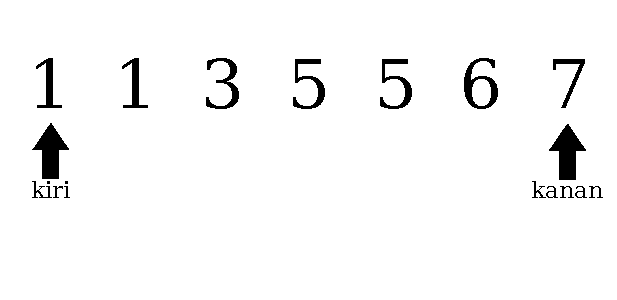
\includegraphics{asset/BS-1.pdf}
    \caption{Misalkan hendak dicari angka 3 dari [1, 1, 3, 5, 5, 6, 7]}
  \end{figure}
\end{frame}

\begin{frame}
\frametitle{Ilustrasi Eksekusi Algoritma (lanj.)}
  \begin{figure}
    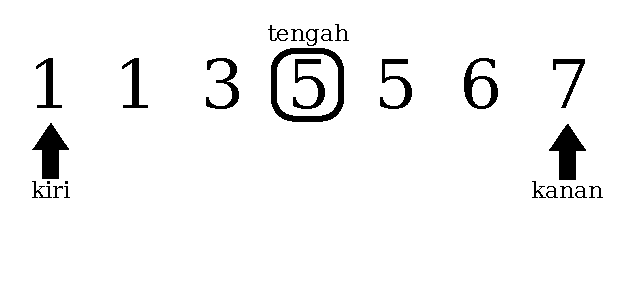
\includegraphics{asset/BS-2.pdf}
    \caption{Angka yang terletak di tengah adalah 5, yang lebih besar dari 3. Artinya, jika angka 3 ada, pasti berada di antara $kiri$ sampai $tengah-1$.}
  \end{figure}
\end{frame}

\begin{frame}
\frametitle{Ilustrasi Eksekusi Algoritma (lanj.)}
  \begin{figure}
    \vspace*{-0.32cm}
    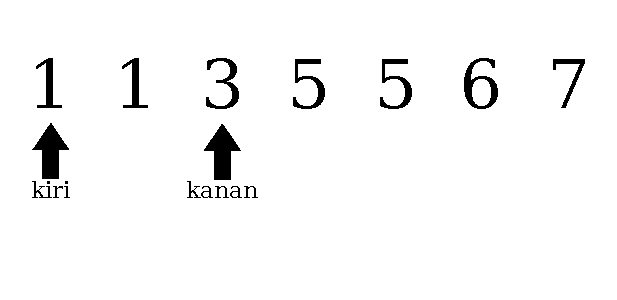
\includegraphics{asset/BS-3.pdf}
    \caption{Sekarang rentang pencarian menjadi hanya separuh dari rentang awalnya.}
  \end{figure}
\end{frame}


\begin{frame}
\frametitle{Ilustrasi Eksekusi Algoritma (lanj.)}
  \begin{figure}
    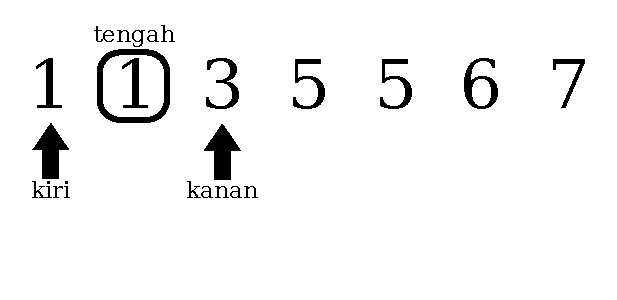
\includegraphics{asset/BS-4.pdf}
    \caption{Angka yang terletak di tengah adalah 1, yang lebih kecil dari 3. Artinya, jika angka 3 ada, pasti berada di antara $tengah+1$ sampai $kanan$.}
  \end{figure}
\end{frame}


\begin{frame}
\frametitle{Ilustrasi Eksekusi Algoritma (lanj.)}
  \begin{figure}
    \vspace*{-0.32cm}
    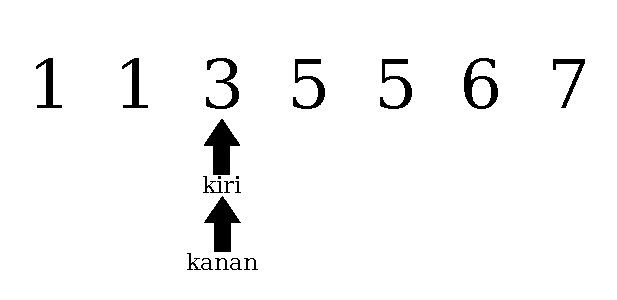
\includegraphics{asset/BS-5.pdf}
    \caption{Kini rentang pencariannya menjadi tinggal satu elemen.}
  \end{figure}
\end{frame}


\begin{frame}
\frametitle{Ilustrasi Eksekusi Algoritma (lanj.)}
  \begin{figure}
    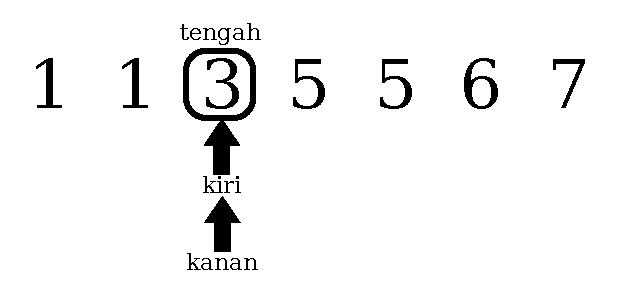
\includegraphics{asset/BS-6.pdf}
    \caption{Ternyata elemen di tengah adalah angka 3, yaitu angka yang dicari. Dengan demikian, angka 3 ditemukan.}
  \end{figure}
\end{frame}


\begin{frame}
\frametitle{Rangkuman}
\begin{block}{Sequential Search}
\begin{itemize}
  \item Data untuk pencarian tidak perlu terurut.
  \item Kompleksitasnya $O(N)$, dengan $N$ adalah ukuran data.
  \item Baik diimplementasikan jika pencarian hanya dilakukan sesekali.
\end{itemize}
\end{block}

\vfill
\begin{block}{Binary Search}
\begin{itemize}
  \item Data untuk pencarian harus terurut.
  \item Kompleksitasnya $O(\log{N})$, dengan $N$ adalah ukuran data.
  \item Baik diimplementasikan jika pencarian perlu dilakukan berkali-kali.
\end{itemize}
\end{block}
\end{frame}

\begin{frame}
\frametitle{Data Tidak Terurut?}
\begin{itemize}
  \item Bagaimana jika kita memiliki data yang sangat banyak, tidak terurut, dan butuh pencarian yang efisien?
  \item Salah satu solusinya adalah dengan \alert{mengurutkan} data tersebut, lalu mengaplikasikan \textit{binary search} untuk setiap pencarian.
  \item Pengurutan akan dipelajari pada materi berikutnya.
\end{itemize}
\end{frame}

\end{document}
